\chapter{ಸುಪ್ರಸಿದ್ಧ ಮಾಯಾಚೌಕಗಳು}

ಬಹಳ ಹಿಂದಿನ ಕಾಲದಿಂದಲೂ ಮಾಯಾಚೌಕಗಳು ರಚಿಸಲ್ಪಟ್ಟಿವೆ. ವಿವಿಧ ಉದ್ದೇಶಗಳಿಗಾಗಿ ಬಳಸಲ್ಪಟ್ಟಿವೆ. ಅವುಗಳಲ್ಲಿ ಕೆಲವು ಸುಪ್ರಸಿದ್ಧ ಮಾಯಾಚೌಕಗಳ ಅಧ್ಯಯನ ಮಾಡೋಣ.

\section*{ನಾಸಿಕ್ ಮಾಯಾಚೌಕ :}

ಮಹಾರಾಷ್ಟ್ರ ರಾಜ್ಯದ ಪ್ರಸಿದ್ಧ ಕ್ಷೇತ್ರಗಳಲ್ಲಿ ನಾಸಿಕವೂ ಒಂದು. ಗೋದಾವರಿ ನದಿ ದಂಡೆಯಲ್ಲಿರುವ ಸುಂದರ ಸ್ಥಳ. ಪುರಾಣ ಪ್ರಸಿದ್ಧವೂ ಹೌದು. ಈ ನಗರದ ಒಂದು ದೇವಸ್ಥಾನದ ಗೋಡೆಯಲ್ಲಿ ಒಂದು ಮಾಯಾಚೌಕ ಕೆತ್ತಲಾಗಿದೆ. ಅನೇಕ ಜನರ ಕಣ್ಣಿಗೆ ಇದು ಬಿದ್ದಿರಬಹುದಾದರೂ ಯಾರೂ ಅಷ್ಟಾಗಿ ಗಮನ ಕೊಟ್ಟಿರಲಿಲ್ಲ. ಇದೇ ನಗರದಲ್ಲಿ ವಾಸಿಸಿದ್ದ ಕ್ರಿಶ್ಚಿಯನ್ ಧರ್ಮಪ್ರಚಾರಕ ರೆವರೆಂಡ್ ಎ.ಎಚ್. ಫ್ರಾಸ್ಟ್ ಇದನ್ನು ಗುರುತಿಸಿದ. ಇದನ್ನು ಬೆಳಕಿಗೆ ತಂದ. ಕ್ರಿ.ಶ. 1514ರಲ್ಲಿ \textbf{ಆಲ್ ಬ್ರೆಕ್ಟ್ ಡ್ಯೂರರ್} (ಜರ್ಮನಿಯ 16ನೇ ಶತಮಾನದ ನವೋದಯ ಕಲಾವಿದ) ಕೆತ್ತನೆ ಮಾಡಿದ್ದ. 4 ಕ್ರಮವರ್ಗದ ಮಾಯಾಚೌಕಕ್ಕಿಂತ ನಾಸಿಕದ ಮಾಯಾಚೌಕ ಉತ್ತಮವಾಗಿದೆಯೆಂಬ ಅಂಶ ಬಯಲಾಯಿತು. ಅಜ್ಞಾತವಾಗಿದ್ದ ಮಾಯಾಚೌಕ \textbf{‘‘ನಾಸಿಕ ಮಾಯಾಚೌಕ’’} ವೆಂದು ಪ್ರಸಿದ್ಧವಾಯಿತು. ಈ ಮಾಯಾಚೌಕವನ್ನು ಕೆಳಗೆ ಕೊಡಲಾಗಿದೆ. ಹೋಲಿಕೆಗಾಗಿ ಡ್ಯೂರರ್ ಚೌಕವನ್ನು ಕೊಟ್ಟಿದೆ.(ಡ್ಯೂರರ್ ಚೌಕದ ವಿವರಗಳು ಚಿತ್ರ V. 3 ರಲ್ಲಿದೆ)
\begin{figure}[H]
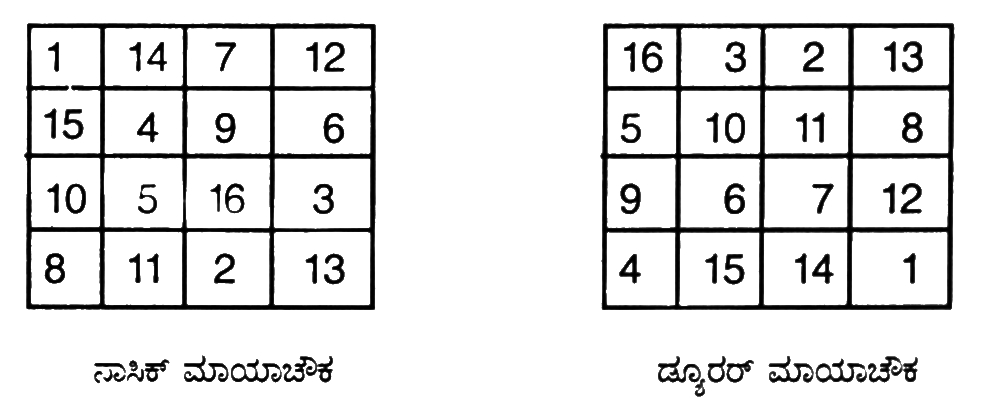
\includegraphics{src/figures/chap4/fig4-1.jpg}
\end{figure}
\begin{figure}[H]
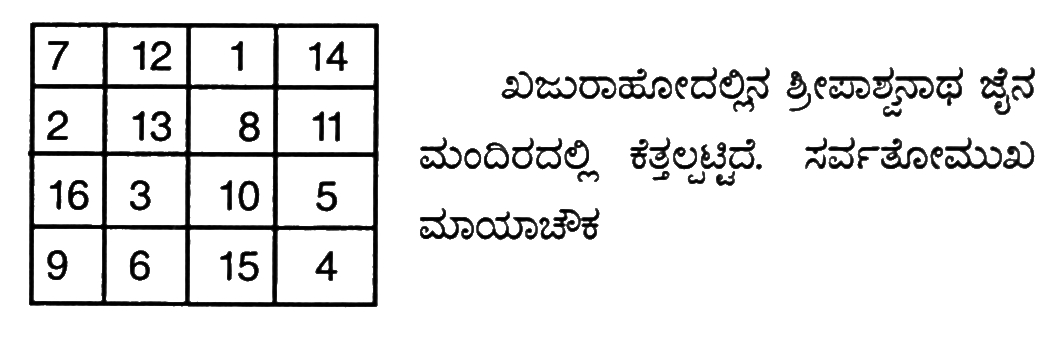
\includegraphics[scale=.9]{src/figures/chap4/fig4-2.jpg}
\end{figure}

\textbf{ನಾಸಿಕ್ ಮಾಯಾಚೌಕದ ಲಕ್ಷಣಗಳು :}

\begin{itemize}
	\item ಅಡ್ಡಸಾಲು, ಕಂಭಸಾಲು, ಕರ್ಣ - ಇವುಗಳ ಪ್ರತಿಯೊಂದರ ಮೊತ್ತ 34
	\item ನಾಲ್ಕು ಮೂಲೆಗಳಲ್ಲಿರುವ ಸಂಖ್ಯೆಗಳ ಮೊತ್ತ 34 (1+12+8+13)
	\item ಯಾವುದೇ $2 \times 2$ಚೌಕದ ಸಂಖ್ಯೆಗಳ ಮೊತ್ತ 34 ಉದಾ: (4+9+5+16), (10+5+8+11)
	\item ಉಪಕರ್ಣಗಳಲ್ಲಿನ ಸಂಖ್ಯೆಗಳ ಮೊತ್ತ 34.

	1+11+16+6; 12+15+5+2; 8+14+9+3; 13+10+4+7; 15+14+2+3; 10+11+7+6
	\item ಈ ರೀತಿ ಅಡ್ಡಸಾಲು, ಕಂಭಸಾಲು, ಕರ್ಣಗಳು, ಉಪಕರ್ಣಗಳು - ಇವುಗಳ ಮೊತ್ತ ಮಾಯಾಮೊತ್ತಕ್ಕೆ ಸಮನಾದರೆ, ಅಂತಹ ಮಾಯಾಚೌಕಕ್ಕೆ  \textbf{‘‘ಸರ್ವತೋಮುಖ ಮಾಯಾಚೌಕ’’ (Pandiagonal Magic Square)} ಎಂಬ ಹೆಸರು.

	(ಗಮನಿಸಿ. ಡ್ಯೂರರ್ ಮಾಯಾಚೌಕವು ಸರ್ವತೋಮುಖ ಮಾಯಾಚೌಕವಲ್ಲ.)
	\item ನಾಸಿಕ್ ಮಾಯಾಚೌಕದ ಕೊನೆಯ ಅಡ್ಡಸಾಲನ್ನು ಮೇಲಕ್ಕೆ ವರ್ಗಾಯಿಸಿ ಬರೆದರೆ ಲಭಿಸುವುದು ಒಂದು ಸರ್ವತೋಮುಖ ಮಾಯಾಚೌಕ. ಈ ಚೌಕದ ಕೊನೆಯ ಸಾಲನ್ನು ಮೇಲಕ್ಕೆ ವರ್ಗಾಯಿಸಿದರೂ, ಸರ್ವತೋಮುಖ ಮಾಯಾಚೌಕವೇ ಬರುತ್ತದೆ. ಹೀಗೆಯೇ ಒಂದೊಂದು ಬಾರಿಗೆ ಒಂದೊಂದು ಕೊನೆಯ ಸಾಲನ್ನು ಮೇಲಕ್ಕೆ ವರ್ಗಾಯಿಸಿದಾಗಲೂ, ಮತ್ತು ಬಲಕೊನೆಯ ಕಂಭಸಾಲನ್ನು ಮೊದಲ ಕಂಭಸಾಲು ಮಾಡಿದಾಗಲೂ, ಮುಂದುವರಿಸಿ ಕೊನೆಯ ಕಂಭಸಾಲನ್ನು ಮೊದಲ ಜಾಗಕ್ಕೆ ವರ್ಗಾಯಿಸಿದಾಗಲೂ ಪ್ರತಿಬಾರಿಯೂ ಸರ್ವತೋಮುಖ ಮಾಯಾಚೌಕ ದೊರೆಯುತ್ತವೆ. ಇವುಗಳನ್ನು ಕೆಳಗಿನ ಚಿತ್ರಗಳು ಸ್ಪಷ್ಟವಾಗಿಸುತ್ತವೆ.
	\begin{figure}[H]
	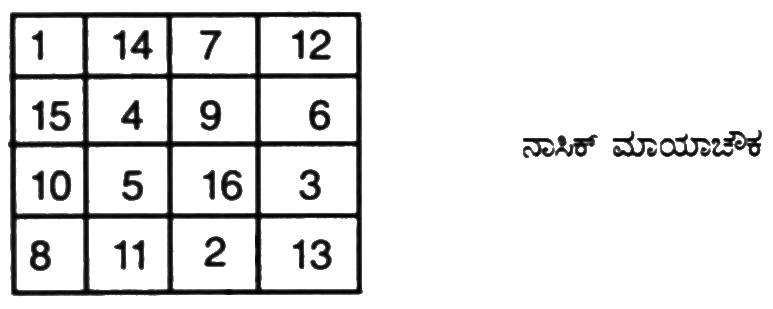
\includegraphics[scale=.8]{src/figures/chap4/fig4-3.jpg}
	\end{figure}
	\begin{figure}[H]
	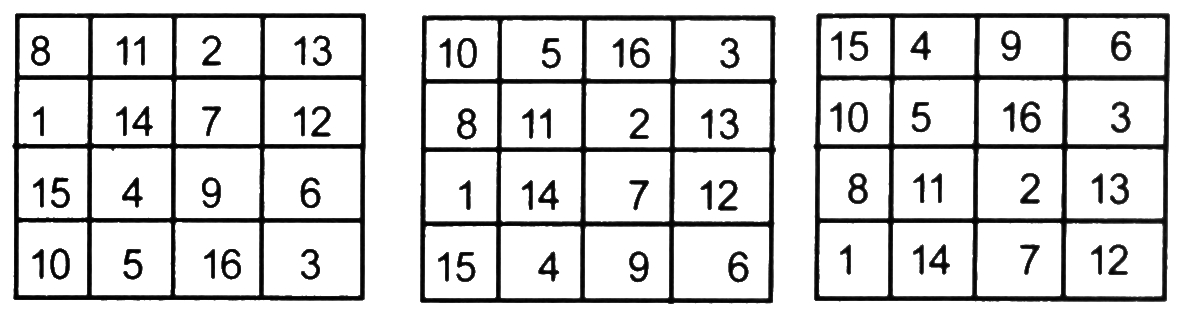
\includegraphics[scale=.8]{src/figures/chap4/fig4-4.jpg}
	\end{figure}

	ಮೇಲಿನ ಚೌಕಗಳಲ್ಲಿ ಅಡ್ಡಸಾಲುಗಳನ್ನು ಒಂದೊಂದರಂತೆ ಮೇಲಕ್ಕೆ ವರ್ಗಾಯಿಸಿದೆ.
	\begin{figure}[H]
	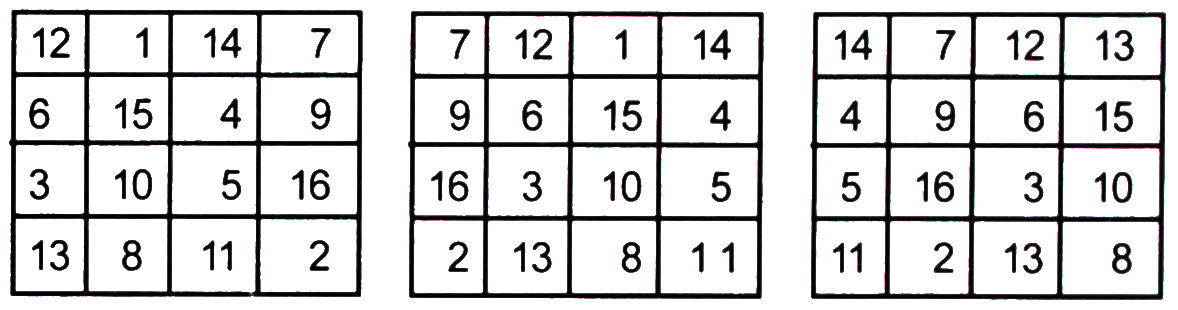
\includegraphics[scale=.8]{src/figures/chap4/fig4-5.jpg}
	\end{figure}
	
	ಮೇಲಿನ ಚೌಕಗಳಲ್ಲಿ ಬಲಕೊನೆಯ ಕಂಭಸಾಲನ್ನು ಒಂದೊಂದರಂತೆ ಎಡಕ್ಕೆ ವರ್ಗಾಯಿಸಿದೆ.
	\item ನಾಸಿಕ್ ಮಾಯಾಚೌಕದ ಮತ್ತೊಂದು ಲಕ್ಷಣವೆಂದರೆ, ಯಾವುದೇ $2 \times 2$ಚೌಕದಲ್ಲಿನ ಸಂಖ್ಯೆಗಳನ್ನು ಕೂಡಿಸಿದರೆ ಮೊತ್ತ 34 ಬರುತ್ತದೆ.
	\item ನಾಲ್ಕು ನಾಸಿಕ್ ಮಾಯಾಚೌಕಗಳನ್ನು ಪರಸ್ಪರ ಲಗತ್ತಾಗುವಂತೆ ಜೋಡಿಸಿ ($8 \times 8$ಚೌಕ ಬರುವಂತೆ) ಬರುವ ರಚನೆಯಲ್ಲಿ ಒಂದು ವಿಶೇಷವಿದೆ. ಒಂದು ರಟ್ಟಿನಲ್ಲಿ $4 \times 4$ ಮನೆಗಳ ಅಳತೆಯ ಒಂದು ಕಿಂಡಿ ಮಾಡಿ. ಇದನ್ನು ಮೇಲಿನ ರಚನೆಯ ಯಾವ ಭಾಗದಲ್ಲಿ ಇಟ್ಟರೂ ಬರುವ $4 \times 4$ ಚೌಕವು ಸರ್ವತೋಮುಖ ಮಾಯಾಚೌಕವಾಗಿರುತ್ತದೆ. ಕೆಳಗಿನ ಚಿತ್ರದಲ್ಲಿ ಅಂತಹ ರಚನೆ ಮತ್ತು ಒಂದು $4 \times 4$ ಚೌಕವನ್ನು ಮಸುಕು ಮಾಡಿ (Shaded)ತೋರಿಸಿದೆ.
	\begin{figure}[H]
	\includegraphics[scale=.7]{src/figures/chap4/fig4-6.eps}
	\end{figure}
\end{itemize}

ನಾಸಿಕ್ ಮಾಯಾಚೌಕದಂತಹುದೇ ಮತ್ತೊಂದು ಮಾಯಾಚೌಕವು ಝಾನ್ಸಿ ಜಿಲ್ಲೆಯ ದುಧೈಯ ಎಂಬಲ್ಲಿನ ಛೋಟಾ ಸುರಂಗ್ ದೇವಾಲಯದ ಚೌಕಟ್ಟಿನಲ್ಲಿರುವುದು ಕಂಡು ಬಂದಿದೆ. ಇದು ಅನೇಕ ಶತಮಾನಗಳಷ್ಟು ಪ್ರಾಚೀನವೆಂದು ಹೇಳಲಾಗಿದೆ. ಅವಗಾಹನೆಗಾಗಿ ಈ ಕೆಳಗೆ ಕೊಟ್ಟಿದೆ. ಅದರ ಲಕ್ಷಣಗಳನ್ನು ಗಮನಿಸಿ.
\begin{figure}[H]
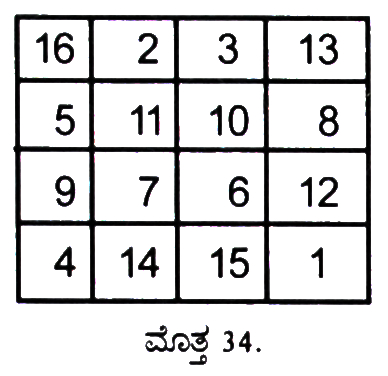
\includegraphics{src/figures/chap4/fig4-7.jpg}
\end{figure}

\subsection*{V. 2. ಮಾನದೇವ ಮಾಯಾಚೌಕ :}

ಅನೇಕ ಶತಮಾನಗಳ ಹಿಂದೆಯೇ ಭಾರತದಲ್ಲಿ ಮಾಯಾಚೌಕಗಳು ಪ್ರಚಲಿತವಾಗಿದ್ದುವು. ಮಾನದೇವ ಸೂರಿ ಎಂಬ ಜೈನ ಕವಿಯ ಒಂದು ಕೃತಿ ‘ಲಘು ಶಾಂತಿ ಸ್ತೋತ್ರ’. ಇದರಲ್ಲಿ ಯಾಂತ್ರಿಕ ಬೀಜಾಕ್ಷರಗಳಿರುವ ಒಂದು ಮಾಯಾಚೌಕವಿದೆ.
\begin{figure}[H]
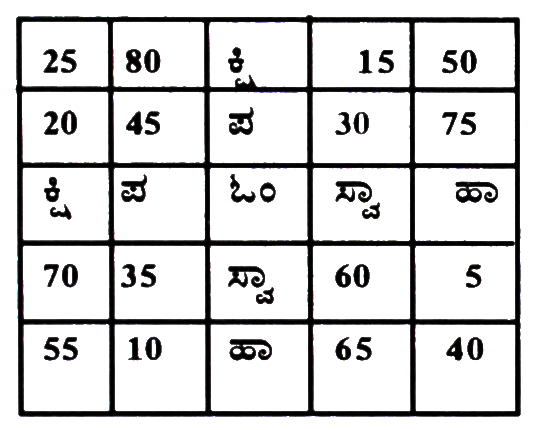
\includegraphics{src/figures/chap4/fig4-8.jpg}
\end{figure}
ಇದರಲ್ಲಿನ ಧಾರ್ಮಿಕ ವಿಚಾರವನ್ನು ನಾವು ಚರ್ಚಿಸುವುದು ಬೇಡ. ಗಣಿತೀಯ ಭಾಗವಾದ ಸಂಖ್ಯೆಗಳನ್ನು ಒಂದು ಚೌಕದಲ್ಲಿ ಬರೆದು ಪರಿಶೀಲಿಸೋಣ. ಎಲ್ಲ ಸಂಖ್ಯೆಗಳೂ 5ರ ಗುಣಕಗಳೆಂಬುದು ವೇದ್ಯವಾಗುತ್ತದೆ. 5ರಿಂದ ಪ್ರತಿ ಸಂಖ್ಯೆಯನ್ನೂ ಭಾಗಿಸಿ, ಭಾಗಲಬ್ಧಗಳನ್ನು $4 \times 4$ ಚೌಕದಲ್ಲಿ ತುಂಬಿಸಿದರೆ, ನಾಲ್ಕು ಕ್ರಮವರ್ಗದ ಮಾಯಾಚೌಕ ಲಭಿಸುತ್ತದೆ.
\begin{figure}[H]
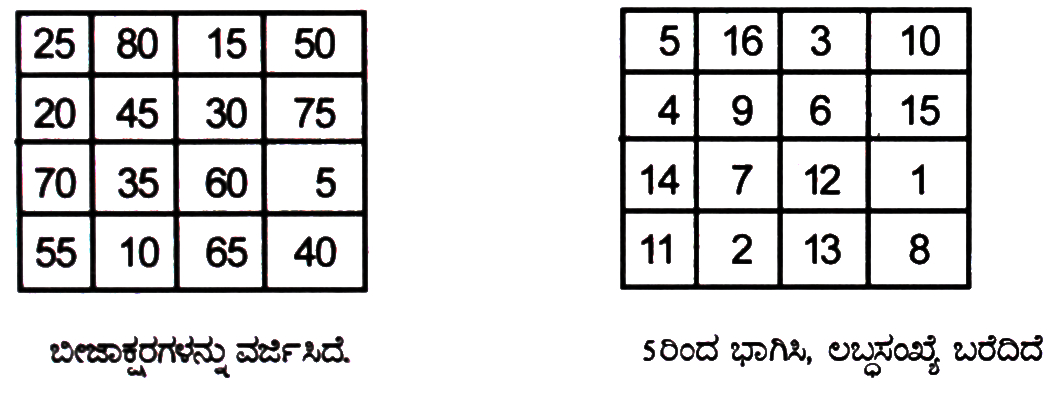
\includegraphics{src/figures/chap4/fig4-9.jpg}
\end{figure}

ಈ ಮಾಯಾಚೌಕವು ‘‘ಸರ್ವತೋಮುಖ ಮಾಯಾಚೌಕ’’ ಇದರ ಮೊದಲ ಕಂಭ ಸಾಲನ್ನು ಕೊನೆಗೆ ವರ್ಗಾಯಿಸಿದರೆ, ಬರುವುದೂ ಒಂದು ಸರ್ವತೋಮುಖ ಮಾಯಾಚೌಕವೇ. ಅಡ್ಡಸಾಲುಗಳನ್ನು ವರ್ಗಾಯಿಸಿದಾಗಲೂ ಸರ್ವತೋಮುಖ ಮಾಯಾಚೌಕಗಳೇ ಲಭಿಸುತ್ತವೆ. ಅಂದರೆ ಒಂದು ಮಾನದೇವ ಚೌಕದ ಅಡ್ಡಸಾಲು, ಕಂಭಸಾಲುಗಳನ್ನು ವರ್ಗಾಯಿಸಿ ಯಾವುದೇ ಸಂಖ್ಯೆಯನ್ನು ಎಡ ಮೇಲ್ತುದಿಯ ಮನೆಗೆ ಬರುವಂತೆ ಮಾಡಬಹುದು. ಹಾಗಾಗಿ ಒಂದು ಮಾನದೇವ ಮಾಯಾಚೌಕದಿಂದ ಹದಿನಾರು ಬೇರೆ ಬೇರೆ ವಿಕಲ್ಪ ರೂಪಗಳನ್ನು ಪಡೆಯಬಹುದು ಎಂದಾಯಿತು.

ಈ ಕೆಳಗೆ ಕೊಟ್ಟಿರುವುಗಳನ್ನು ಮೂಲಭೂತ ಸರ್ವತೋಮುಖ ಮಾಯಾಚೌಕಗಳೆನ್ನಲಾಗಿದೆ.
\begin{figure}[H]
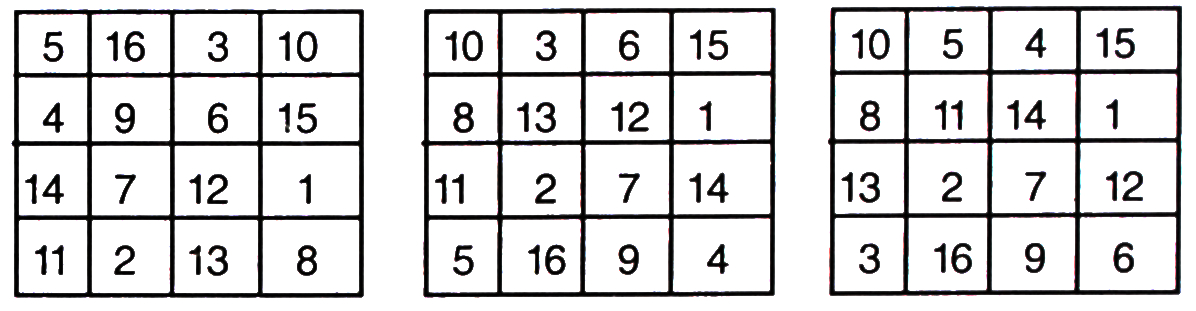
\includegraphics{src/figures/chap4/fig4-10.jpg}
\end{figure}

ಈ ಮೂರು ಸರ್ವತೋಮುಖ ಮಾಯಾಚೌಕಗಳಿಂದ ಸ್ಥಳಾಂತರ ಮೂಲಕ, ಒಂದೊಂದರಿಂದಲೂ 16 ಚೌಕಗಳಂತೆ, ಒಟ್ಟು 48 ಸರ್ವತೋಮುಖ ಮಾಯಾಚೌಕಗಳನ್ನು ಪಡೆಯಬಹುದು. ಹೀಗೆ ಲಭಿಸಿದ 48 ಮಾಯಾಚೌಕಗಳಲ್ಲಿ ಪ್ರತಿಯೊಂದನ್ನೂ ಕಾಲು ಸುತ್ತು, ಅರ್ಧಸುತ್ತು, ಮುಕ್ಕಾಲು ಸುತ್ತು ತಿರುಗಿಸಿ ಹಾಗೂ ಅವುಗಳನ್ನು ಪ್ರತಿಬಿಂಬಿಸಿ 8 ಬೇರೆ ಬೇರೆ ರೂಪಗಳನ್ನು ಪಡೆಯಬಹುದು. ಅಂದರೆ ಒಟ್ಟಾರೆ $48 \times 8$=384ರ ಸರ್ವತೋಮುಖ ಮಾಯಾಚೌಕಗಳನ್ನು ಪಡೆಯಬಹುದು. ಉದಾಹರಣೆಗೆ ಒಂದು ಚೌಕವನ್ನು ತಿರುಗಿಸಿ ಮತ್ತು ಅದರ ಪ್ರತಿಬಿಂಬ ಕೊಟ್ಟಿದೆ. $a, b, c, d$ ಮಾಯಾಚೌಕಗಳು $A, B, C, D$ ಪ್ರತಿಬಿಂಬಗಳು
\begin{figure}[H]
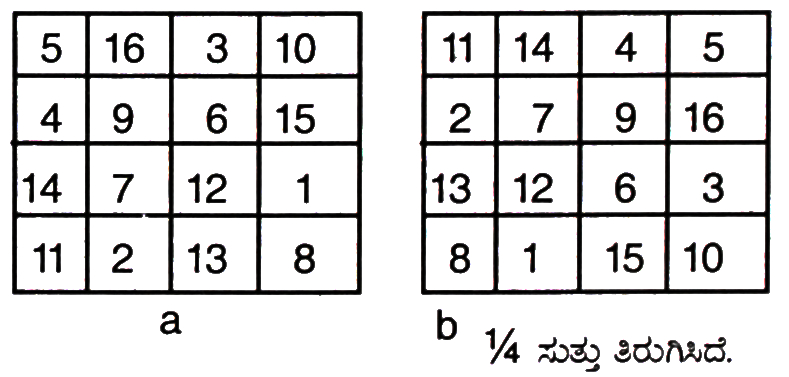
\includegraphics{src/figures/chap4/fig4-11.jpg}
\end{figure}
\begin{figure}[H]
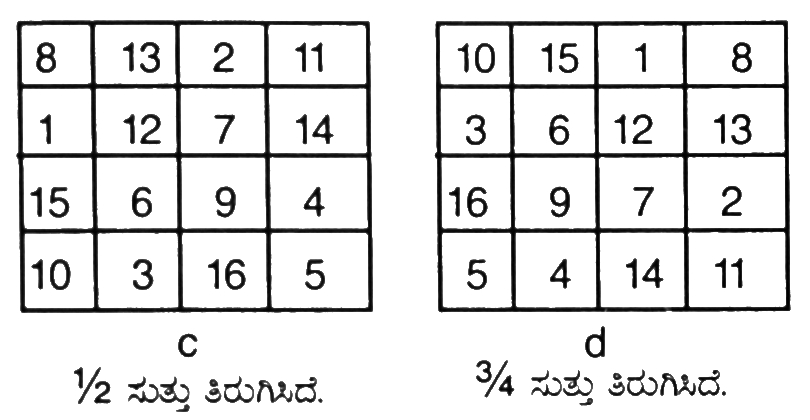
\includegraphics{src/figures/chap4/fig4-12.jpg}
\end{figure}
\begin{figure}[H]
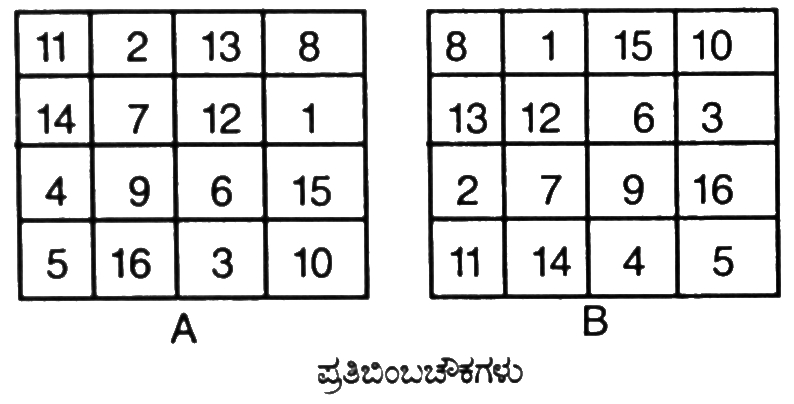
\includegraphics{src/figures/chap4/fig4-13.jpg}
\end{figure}
\begin{figure}[H]
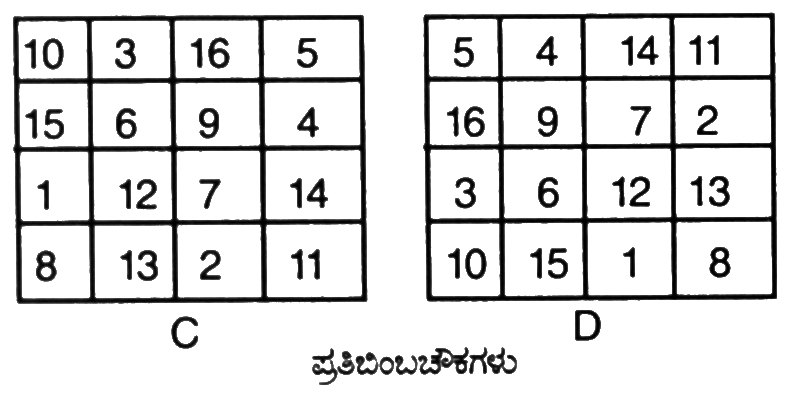
\includegraphics{src/figures/chap4/fig4-14.jpg}
\end{figure}

ಈ ಚೌಕಗಳಲ್ಲಿಯ ಸಂಖ್ಯೆಗಳನ್ನು ಸ್ಥಳಾಂತರಿಸಿ 880 ಬೇರೆ ಬೇರೆ ಮಾಯಾಚೌಕಗಳನ್ನು ಪಡೆಯಬಹುದೆಂದು ಲೆಕ್ಕ ಹಾಕಲಾಗಿದೆ.
\begin{center}
*****
\end{center}

\subsection*{V. 3. ಡ್ಯೂರರ್ ಮಾಯಾಚೌಕ}

ಆಲ್ಬ್ರೆಕ್ಟ್ ಡ್ಯೂರರ್ ಜರ್ಮನಿಯ ಕಲಾವಿದರಲ್ಲೊಬ್ಬ. 16ನೆಯ ಶತಮಾನದಲ್ಲಿದ್ದವನು. ನವೋದಯ ಅಥವಾ ಕಲಾಪುನರುಜ್ಜೀವನ ಅವಧಿಯಲ್ಲಿ. ಆ ಕಾಲದಲ್ಲಿ ಅತಿ ಪ್ರಸಿದ್ಧ ಕಲಾವಿದನೆಂಬ ಹೆಸರು ಗಳಿಸಿದ್ದ.ಆತನ ಕೆತ್ತನೆ ಶಿಲ್ಪಗಳಲ್ಲಿ \textbf{‘‘ಖಿನ್ನತೆ’’ (Melancholia I)} ಎಂಬುದೊಂದು. ಇದರಲ್ಲಿನ ಅನೇಕ ಅಂಶಗಳು ವಿದ್ವಾಂಸರನ್ನು ಶತಮಾನಗಳಷ್ಟು ಕಾಡಿವೆ. ತನ್ನ ಅಪೂರ್ಣ ಕಲಾಕೃತಿಗಳ ಮಧ್ಯೆ ಚಿಂತಾಕ್ರಾಂತಳಾಗಿ ಕುಳಿತಿರುವ ಮಹಿಳೆಯನ್ನು ಕಾಣುತ್ತೇವೆ. ಸುತ್ತಮುತ್ತ ಉಪಕರಣಗಳು ಚೆಲ್ಲಾಪಿಲ್ಲಿಯಾಗಿವೆ. ಮರಳು ಗಡಿಯಾರ ಮೂಡಿಬಂದಿದೆ. ಬಲ ಮೇಲ್ತುದಿಯಲ್ಲಿ ಒಂದು ಗಂಟೆ ಕೆತ್ತಲಾಗಿದೆ. ಅದರ ಕೆಳಗೆ ಮಾಯಾಚೌಕ ಕಾಣಿಸುತ್ತದೆ. ಗಂಟೆಗೆ ಆನಿಸಿದಂತೆ ತಕ್ಕಡಿ ಇದೆ. ಪಂಡಿತರ ವಿಶ್ಲೇಷಣೆಯಂತೆ ಈ ಕೆತ್ತನೆಯು ದೈವಿಕ ಸತ್ಯವನ್ನು ಸಾಕ್ಷಾತ್ಕಾರಿಸುವ ಹಾಗೂ ನಿಸರ್ಗದ ರಹಸ್ಯಗಳನ್ನು ಬಯಲು ಮಾಡುವ ಮಾನವನ ಅಸಫಲ ಯತ್ನಗಳ ಪ್ರತೀಕವಾಗಿದೆ.

ಆ ಕಾಲದ ಜ್ಯೋತಿಷಿಗಳು 4 ಕ್ರಮವರ್ಗದ ಮಾಯಾಚೌಕಗಳನ್ನು ‘ಗುರು’ ಗ್ರಹಕ್ಕೆ ಸಂಬಂಧಿತವೆಂದೂ, ಶನಿಗ್ರಹದಿಂದ ಉಂಟಾಗುವ ಖಿನ್ನತೆಯನ್ನು ನಿವಾರಿಸುವುದೆಂದೂ ನಂಬಿದ್ದರು.
\begin{figure}[H]
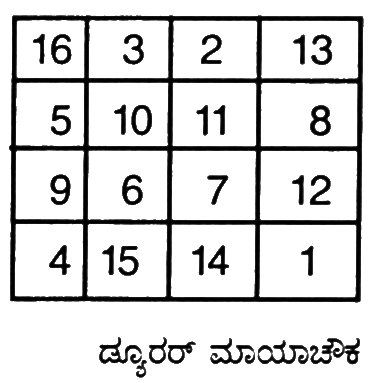
\includegraphics{src/figures/chap4/fig4-15.jpg}
\end{figure}
\begin{itemize}
	\item ಇದರಲ್ಲಿ 1 ರಿಂದ 16 ವರೆಗೆ ಕ್ರಮಾಗತ ಸಂಖ್ಯೆಗಳನ್ನು ಬಳಸಲಾಗಿದೆ.
	\item ಅಡ್ಡಸಾಲು, ಕಂಭಸಾಲು ಮತ್ತು ಕರ್ಣಗಳ ಮನೆಗಳ ಸಂಖ್ಯೆಗಳ ಮೊತ್ತ 34
	\item ನಾಲ್ಕು ಮೂಲೆಗಳಲ್ಲಿನ ಸಂಖ್ಯೆಗಳ ಹಾಗೂ ಮಧ್ಯದ ನಾಲ್ಕು ಮನೆಗಳಲ್ಲಿನ ಸಂಖ್ಯೆಗಳ ಮೊತ್ತವೂ 34.
	\item ಸಮಖಂಡದ ಉಪಕರ್ಣಗಳ ಸಂಖ್ಯೆಗಳ ಮೊತ್ತ 34. ಸಮಖಂಡದ ಉಪಕರ್ಣ ವೆಂದರೆ ಒಂದು ಖಂಡವು ಎರಡು ಮನೆಗಳ ಮೇಲೂ ಮತ್ತೊಂದು ಖಂಡವು ಇತರ ಎರಡು ಮನೆಗಳ ಮೇಲೂ ಹಾದು ಹೋಗುವುದು.

	ಉದಾ: 5+3 ಒಂದು ಖಂಡ, 14+12 ಇನ್ನೊಂದು ಖಂಡ. ಇವುಗಳ ಮೊತ್ತ 34 ಇದೇ ರೀತಿ 9+15 ಮತ್ತು 2+8 ಇವುಗಳ ಮೊತ್ತವೂ 34.
	\item ಈ ಕೆಳಗಿನ ಚಿತ್ರಗಳಲ್ಲಿರುವ ಆಕೃತಿಗಳನ್ನು ಗಮನಿಸಿ. ಅವುಗಳ ನಾಲ್ಕು ಶೃಂಗಗಳ ಸ್ಥಾನದಲ್ಲಿ ಬರುವ ಡ್ಯೂರರ್ ಚೌಕದ ನಾಲ್ಕು ಸಂಖ್ಯೆಗಳ ಮೊತ್ತ 34.
	\begin{figure}[H]
	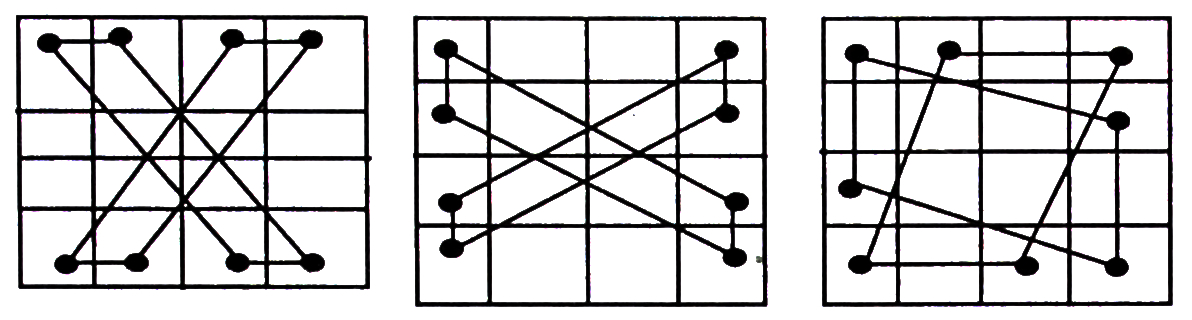
\includegraphics{src/figures/chap4/fig4-16.jpg}
	\end{figure}
	\begin{figure}[H]
	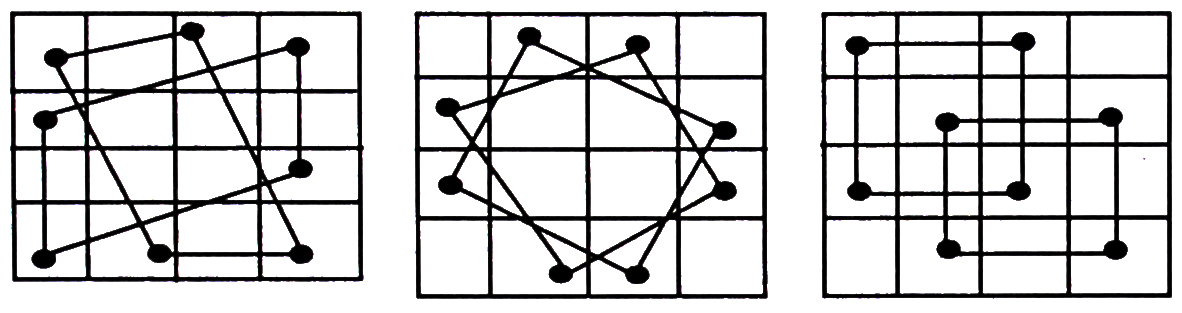
\includegraphics{src/figures/chap4/fig4-17.jpg}
	\end{figure}
	\begin{figure}[H]
	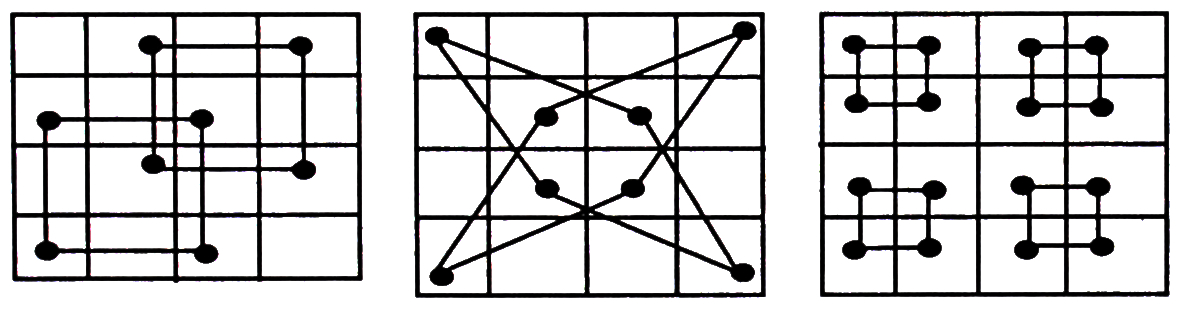
\includegraphics{src/figures/chap4/fig4-18.jpg}
	\end{figure}
	\begin{figure}[H]
	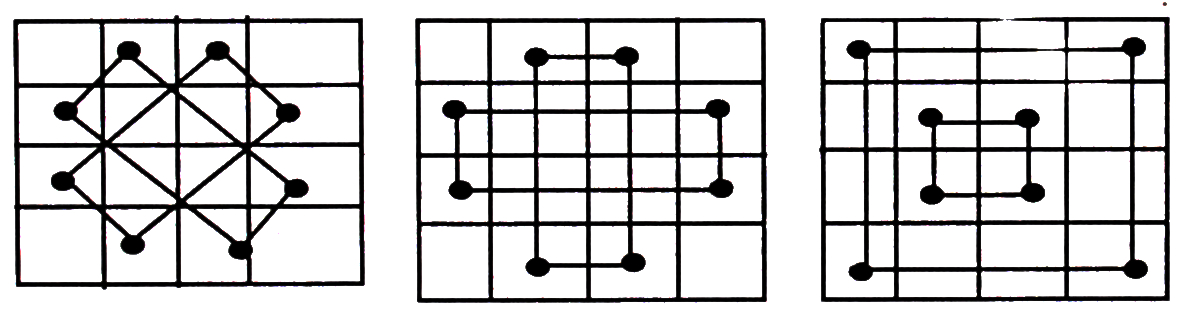
\includegraphics{src/figures/chap4/fig4-19.jpg}
	\end{figure}

	\item ಡ್ಯೂರರ್ ಮಾಯಾಚೌಕದ ಸಂಖ್ಯೆಗಳಲ್ಲಿನ ವರ್ಗ (Square)ಮತ್ತು ಘನ (Cube) ಗಳನ್ನು ಅನುರೂಪಮನೆಗಳಲ್ಲಿ ಬರೆಯೋಣ
	ಈ ಚೌಕವನ್ನು ಪರಿಶೀಲಿಸಿ, ಅದರ ಲಕ್ಷಣಗಳನ್ನು ತಿಳಿಯೋಣ.
	\begin{figure}[H]
	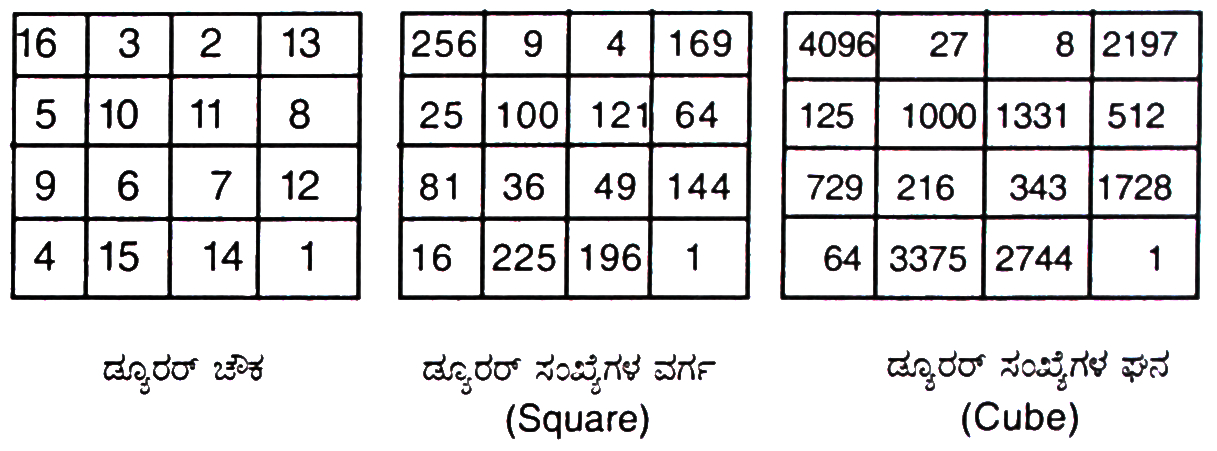
\includegraphics{src/figures/chap4/fig4-20.jpg}
	\end{figure}

	\item ವರ್ಗಚೌಕದಲ್ಲಿ 1 ಮತ್ತು 2ನೆಯ ಅಡ್ಡಸಾಲು ಸಂಖ್ಯೆಗಳ ಮೊತ್ತ 748

	2 ಮತ್ತು 4ನೆಯ ಅಡ್ಡಸಾಲು ಸಂಖ್ಯೆಗಳ ಮೊತ್ತ 748

	3 ಮತ್ತು 4ನೆಯ ಅಡ್ಡಸಾಲು ಸಂಖ್ಯೆಗಳ ಮೊತ್ತ 748

	ಕರ್ಣ ಸಂಖ್ಯೆಗಳನ್ನು ಹೊರತು ಪಡಿಸಿ ಉಳಿದ 8ಸಂಖ್ಯೆಗಳ ಮೊತ್ತ 748
	\item ವರ್ಗಚೌಕದಲ್ಲಿ 1ನೆಯ ಮತ್ತು 2ನೆಯ ಕಂಭಸಾಲು, ಸಂಖ್ಯೆಗಳ ಮೊತ್ತ 748

	2 ಮತ್ತು 3ನೆಯ ಕಂಭಸಾಲು ಸಂಖ್ಯೆಗಳ ಮೊತ್ತ 748

	3ಮತ್ತು 4ನೆಯ ಕಂಭಸಾಲು ಸಂಖ್ಯೆಗಳ ಮೊತ್ತ 748
	\item ಡ್ಯೂರರ್ ಘನ ಚೌಕದಲ್ಲಿ ಕರ್ಣ ಸಂಖ್ಯೆಗಳ ಮೊತ್ತ = ಕರ್ಣೇತರ ಸಂಖ್ಯೆಗಳ ಮೊತ್ತ= 9248

	\item ಡ್ಯೂರರ್ ಚೌಕದ ಕೊನೆ ಅಡ್ಡಸಾಲಿನ ಮಧ್ಯದ 2 ಸಂಖ್ಯೆಗಳನ್ನು ಜೋಡಿಸಿದರೆ 1514 ಆಗುತ್ತದೆ. ಇದು ಡ್ಯೂರರ್ ಈ ಚೌಕವನ್ನು ಕೆತ್ತಿದ ಇಸವಿ ಎಂಬುದು ವಿಸ್ಮಯವಲ್ಲವೇ ?
\end{itemize}

\subsection*{V. 4. ಗ್ವಾಲಿಯರ್ ಮಾಯಾಚೌಕ :}

ಕ್ರಿ.ಶ. 1892ರಲ್ಲಿ ಎಡ್ವರ್ಡ್ ಫಾಕ್ನರ್ ಎಂಬ ಗಣಿತಜ್ಞ 8 ಕ್ರಮವರ್ಗದ ಒಂದು ಮಾಯಾಚೌಕವನ್ನು ಪರಿಚಯಿಸಿದ. ಅದಕ್ಕೆ ಗ್ವಾಲಿಯರ್ ಮಾಯಾಚೌಕ ಅಥವಾ ಭಾರತೀಯ (ಇಂಡಿಯನ್) ಮಾಯಾಚೌಕ ಎಂದು ಹೆಸರಿಸಿದ. ಆ ಸಂದರ್ಭದಲ್ಲಿ ಅವನು ಬರೆದಿರುವುದು ಹೀಗೆ :-

‘‘ಈ ಚೌಕಗಳಿಗೆ ಸೂಕ್ತವಾದ ಹೆಸರು ಭಾರತೀಯ (ಇಂಡಿಯನ್) ಚೌಕಗಳು. ಅಲ್ಲಿನ ಬ್ರಾಹ್ಮಣ ವಿದ್ವಾಂಸರು ಅನೇಕ ಶತಮಾನಗಳಿಂದ ಇಂತಹ ಮಾಯಾ ಚೌಕಗಳನ್ನು ರಚಿಸುವುದರಲ್ಲಿ ಪರಿಣತರು. ಧರ್ಮಪ್ರಚಾರಕ ಎ.ಎಚ್. ಫ್ರಾಸ್ಟರು ಇವುಗಳನ್ನು ಭಾರತೀಯ (ಇಂಡಿಯನ್) ಚೌಕಗಳೆಂದು ಕರೆದಿದ್ದಾರೆ. ಇಂತಹವುಗಳಲ್ಲಿ ಒಂದು ಮಾಯಾಚೌಕವು ಗ್ವಾಲಿಯರ್ ನಗರದ ಕೋಟೆಯ ಹೆಬ್ಬಾಗಿಲಿನ ಮೇಲೆ ಕೆತ್ತಲ್ಪಟ್ಟಿದೆ. ತಾಯಿತಗಳಲ್ಲಿ ಇವುಗಳನ್ನು ಬರೆದು ಭಾರತೀಯರು ಧರಿಸುತ್ತಾರೆ............’’

ಈ ಚೌಕವನ್ನು ಪರಿಶೀಲಿಸಿ, ಅದರ ಲಕ್ಷಣಗಳನ್ನು ತಿಳಿಯೋಣ.
\begin{figure}[H]
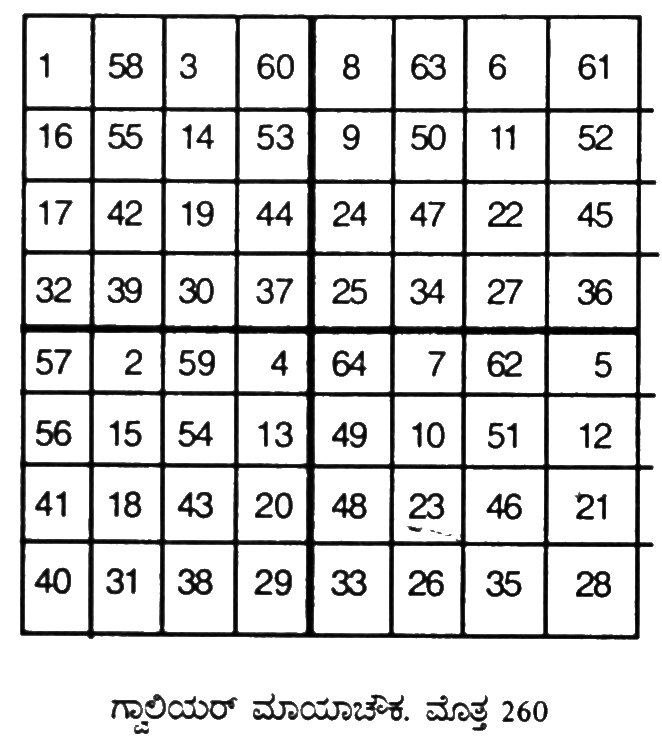
\includegraphics{src/figures/chap4/fig4-21.jpg}
\end{figure}

\textbf{ಲಕ್ಷಣಗಳು :}

\begin{itemize}
	\item 8 ಕ್ರಮವರ್ಗದ ಮಾಯಾಚೌಕ.1ರಿಂದ 64ರ ವರೆಗೆ ಕ್ರಮಾಗತಸಂಖ್ಯೆಗಳನ್ನು ಬಳಸಿದೆ.
	\item ಅಡ್ಡಸಾಲು, ಕಂಭಸಾಲು, ಕರ್ಣಗಳ ಸಂಖ್ಯೆಗಳ ಮೊತ್ತ 260
	\item ಯಾವುದೇ $2 \times 2$ ಚೌಕದ ಸಂಖ್ಯೆಗಳ ಮೊತ್ತ 130.
	\item ಕೊನೆಯ ಅಡ್ಡಸಾಲನ್ನು ಮೇಲಕ್ಕೆ ವರ್ಗಾಯಿಸಿದಾಗ ಮಾಯಾಚೌಕದ ಲಕ್ಷಣಗಳು ಬದಲಾಗುವುದಿಲ್ಲ
	\item ಬಲ ಕೊನೆಯ ಕಂಭಸಾಲನ್ನು ಎಡಗಡೆಗೆ ವರ್ಗಾಯಿಸಿ ಮೊದಲ ಕಂಭಸಾಲನ್ನಾಗಿ ಮಾಡಿದರೂ ಮಾಯಾಚೌಕದ ಲಕ್ಷಣಗಳು ಬದಲಾಗುವುದಿಲ್ಲ.
	\item ಮಾಯಾಚೌಕವನ್ನು ನಾಲ್ಕು ಸಮಭಾಗಗಳಾಗಿ ಮಾಡಿ. ಕರ್ಣಾಭಿಮುಖ (Diagonally Opposite) ಚೌಕಗಳಲ್ಲಿನ ಅನುರೂಪ (Corresponding) ಮನೆಗಳ ಸಂಖ್ಯೆಗಳ ಮೊತ್ತ 65.

	ಉದಾ : 1+64, 58+7, 29+36 ಇತ್ಯಾದಿ
	\item ಯಾವುದೇ 2 ಸಮಾಂತರ ಉಪಕರ್ಣಗಳ ಮನೆಗಳ ಮೊತ್ತ 8 ಆಗುವಂತೆ, ತೆಗೆದುಕೊಂಡ ರೆ, ಆ ಮನೆಗಳ ಸಂಖ್ಯೆಗಳ ಮೊತ್ತ 260
	\begin{figure}[H]
	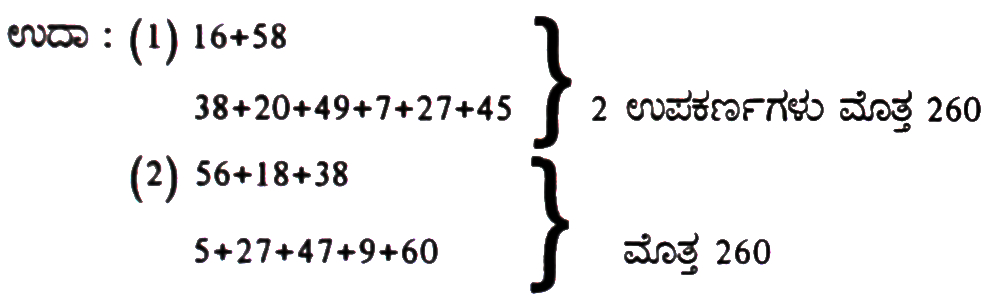
\includegraphics{src/figures/chap4/fig4-22.jpg}
	\end{figure}
\end{itemize}

\subsection*{V. 5. ಜೋಹಾನ್ ಫಾಲ್ ಹಾಬರ್ನ 15 ಕ್ರಮವರ್ಗದ ಚೌಕ :}

17ನೆ ಶತಮಾನದಲ್ಲಿ ಯೂರೋಪಿನ ಹಲವು ಗಣಿತಜ್ಞರು ಮಾಯಾಚೌಕಗಳ ಬಗೆಗೆ ಕೆಲಸ ಮಾಡಿದ್ದುಂಟು. ಅವರಲ್ಲಿ ಜರ್ಮನಿಯ ಜೋಹಾನ್ ಫಾಲ್ ಹಾಬರ್ನೂ ಒಬ್ಬ. ಇವನು ತನ್ನ ಒಂದು ಗ್ರಂಥದಲ್ಲಿ 15 ಕ್ರಮವರ್ಗದ ಒಂದು ಮಾಯಾಚೌಕವನ್ನು ಉದಾಹರಿಸಿದ್ದಾರೆ. ಇದರ ಕರ್ತೃ ಅಜ್ಞಾತ. ಕುತೂಹಲಕಾರಿ ರಚನಾ ವಿಧಾನವಿರುವುದರಿಂದ ಅದನ್ನು ಕೊಟ್ಟಿದೆ.
\begin{itemize}
	\item $15 \times 15$ಚೌಕದ ಮಧ್ಯದ ಮನೆಯ ಬಲಗಡೆ ಮನೆಯಿಂದ ಪ್ರಾರಂಭಿಸಿ. ಡಿ.ಲಾ. ಲೌಬೊರೆ ವಿಧಾನದಿಂದ ಮನೆಗಳನ್ನು ತುಂಬಿಸಿ.
	\item ತುಂಬಿದ ಮನೆ ಎದುರಾದಾಗ ಬಲಗಡೆಗೆ ಎರಡುಮನೆ ಜಿಗಿದು ಮುಂದುವರಿಸಿ.
	\item ಬಲಗಡೆ ಮನೆ ಇಲ್ಲದಿದ್ದಾಗ ಅದೇ ಅಡ್ಡಸಾಲಿನ ಎಡ ತುದಿಯಿಂದ 2 ಮನೆ ಜಿಗಿದು ತುಂಬಿಸಿ. (120 ನಂತರ 121 ತುಂಬಿಸಿರುವುದನ್ನು ನೋಡಿ, 105ರ ನಂತರ 106)
	\item ಮಾಯಾಚೌಕ ಸಿದ್ಧ. ಮೊತ್ತ 1695.
	\begin{figure}[H]
	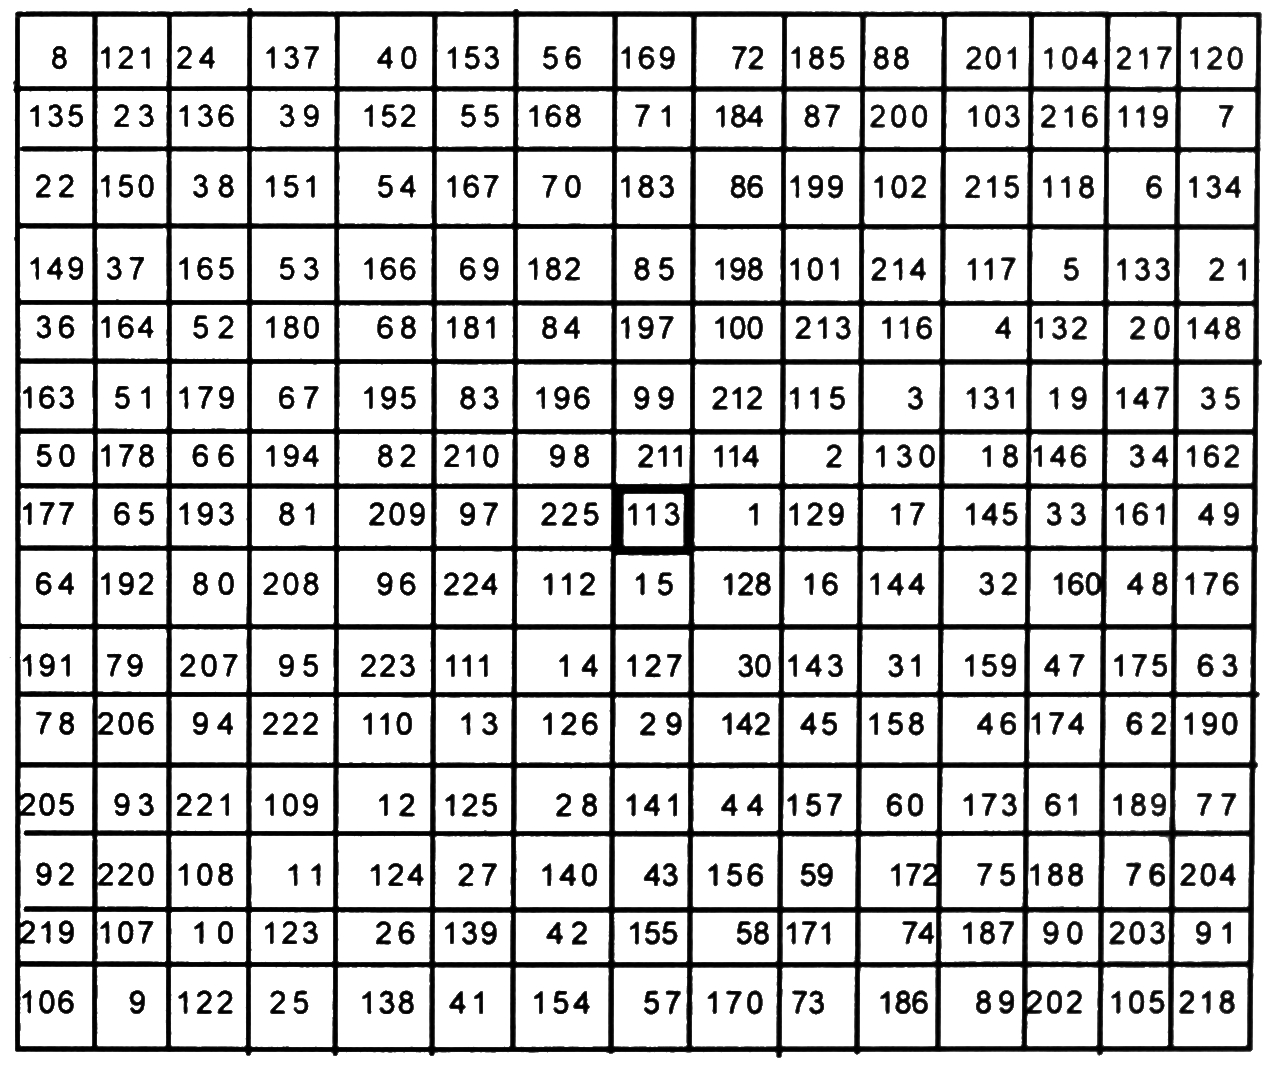
\includegraphics{src/figures/chap4/fig4-23.jpg}
	\end{figure}
\end{itemize}
